\documentclass[
  final,
  babelLanguage=portuguese,
  desktopVersion,
  %showtrims,
  %overleaf,
]{anecdote}

%\graphicspath{{./assets/photos/300dpi/}}
\graphicspath{{./assets/photos/92dpi/}}

% Page size: 6x9 inch
% Body text: 10.5 / 15 pt

\usepackage{local}

%% Details of the book
%% ===================

\title{Destronar o Tirano Interior}
\subtitle{}
\author{Ajahn Sucitto}
\publisher{Publicações Sumedhārāma}
\date{2022-05-22}
\editionInfo{\textit{Primeira edição}, 2022}
\ISBN{978-989-8994-33-2}

% === Metadata ===

\hypersetup{
  pdftitle={\thetitle},
  pdfauthor={\theauthor},
  pdfcopyright={Copyright (C) 2022, \thePublisher},
  pdfsubject={},
  pdfkeywords={},
  pdflicenseurl={https://creativecommons.org/licenses/by-nc-nd/4.0/},
  pdfcontacturl={},
  pdflang={pt},
}

%% === Load further packages ===

%% === Hyphenation exceptions and corrections ===

\hyphenation{London}

\begin{document}

\frontmatter

\ifdesktopversion
\desktopCover{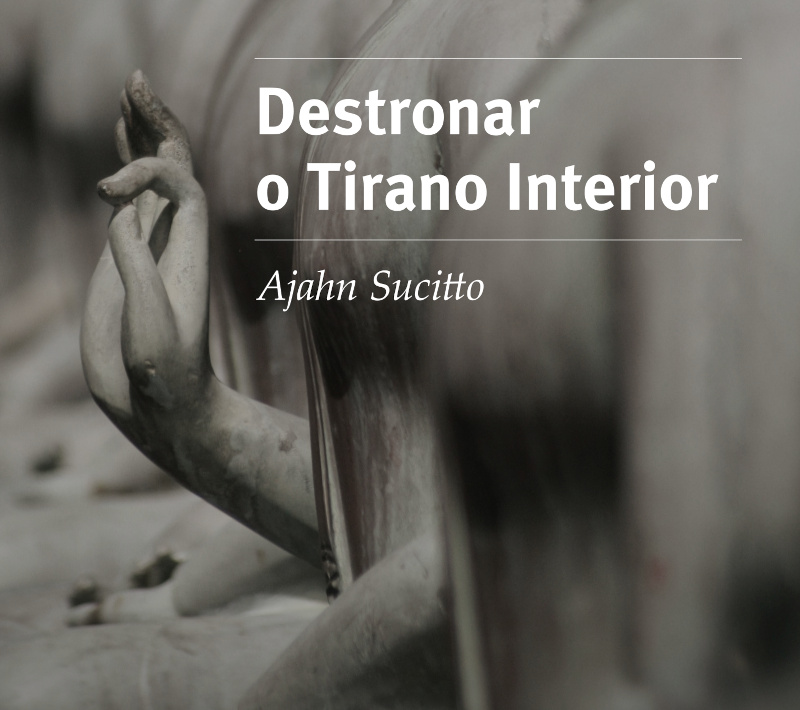
\includegraphics[height=\paperheight]{./desktop-cover.jpg}}
\fi

\cleartorecto
\thispagestyle{empty}
\vspace*{5em}

{\centering

\settowidth{\titleLength}{%
  {\Large\chapterTitleFont\scshape\MakeLowercase{\thetitle}}%
}

{\Large\chapterTitleFont\scshape\MakeLowercase{\thetitle}}\\[0.3\baselineskip]
\setlength{\xheight}{\heightof{X}}
\raisebox{0.5\xheight}{\color[gray]{0.4}\rule{\titleLength}{0.25pt}}\\[0.3\baselineskip]

\vfill

\theauthor

\vspace*{5em}

}



\cleartoverso
\thispagestyle{empty}

\vspace*{-2.5\baselineskip}
\enlargethispage{2.5\baselineskip}

{\fontsize{7}{9}\selectfont
\centering
\setlength{\parindent}{0pt}%
\setlength{\parskip}{6pt}%

\thetitle\\
por \theauthor

Publicações Sumedhārāma\\
\href{https://sumedharama.pt}{www.sumedharama.pt}

Para distribuição gratuita\\
\textit{Sabbadānaṃ dhammadānaṃ jinati}\\
‘A oferta de Dhamma é superior a qualquer outra oferta.’

Este livro encontra-se disponível para distribuição gratuita em:\\
\href{https://sumedharama.pt}{www.sumedharama.pt}\\
\href{https://forestsangha.org}{www.forestsangha.org}

ISBN \theISBN

Copyright \copyright\ Publicações Sumedhārāma 2022

Tradutor: João Brinco\\
Capa: Filipe Dumas\\
Editor: Appamādo Bhikkhu\\
Formatação: Gambhīro Bhikkhu

Publicado originalmente em 2014 pelas Publicações de Amaravati\\
\emph{Unseating the Inner Tyrant}\\
Copyright \copyright\ Amaravati Publications 2014

\vfill

Este trabalho está licenciado com uma Licença Creative Commons\\
Atribuição-NãoComercial-SemDerivações 4.0 Internacional.

Veja página \pageref{copyright-details} para mais detalhes sobre direitos e restrições desta licença.\\
Produzido com o sistema tipográfico \LaTeX. Fonte utilizada: Gentium e Fira~Sans.

\theEditionInfo

}


\cleartorecto

\clearpage
\thispagestyle{empty}

{\sectionFmt{Dedicação do autor}}

\vspace*{0.8\baselineskip}

Pelo meu sexagésimo quinto aniversário, desejo oferecer estes
ensinamentos e qualquer bem que deles advenha, pelo bem dos meus pais,
Charles e Winifred Malcolm. Vocês deram"-me tudo o que tinham.

\clearpage
\thispagestyle{empty}

{\sectionFmt{Dedicação dos patrocinadores}}

\enlargethispage*{\baselineskip}

\vspace*{0.8\baselineskip}

Esta publicação é possível devido à generosidade do Senhor e Senhora N.
de Silva, que a oferecem por gratidão ao Sangha de monges e monjas pela
sua dedicação incondicional ao ensino do Dhamma no ocidente.

Alguma vez te deste conta de estar dominado por uma corrente de
pensamentos que te dizem que não és bom o suficiente, que não mereces
muito, que as outras pessoas te acham inferior, ou que apenas te toleram
por cortesia? Alguma vez dás por ti a ruminar em memórias de coisas que
fizeste mal, ou relações que não funcionaram? Sentes que tens de ter
tanto sucesso quanto achas que os outros têm, criticando"-te a ti próprio
constantemente? Este fenómeno psicológico chama"-se ‘O Tirano Interior’.
As boas notícias são que não és a única pessoa que o tem, e que é
possível escapares ao seu controlo. E a chave para o fazer é
estabelecer, e continuamente reestabelecer, a intenção correcta.



% Page 1 is the first page of the first chapter.
\mainmatter

\chapter{Destronar o Tirano Interior}

\section{Intenção correta}

A intenção é a atitude ou inclinação que forma a base das nossas acções,
e numa vida cheia de coisas com que lidar, é fácil perder essa base. No
entanto, a intenção é importante: ela cria uma tendência e afecta a
forma como vemos a vida, e como agimos ou falamos. Se tivermos uma
intenção negativa, vemos a vida com uma percepção negativa; se limparmos
a nossa mente de intenções hostis ou depressivas, sentimo"-nos leves e
claros, e as nossas acções e palavras estarão de acordo com esse estado
mental. Este é o princípio de causa e efeito, a visão correcta, a pedra
basilar do caminho para transcender o sofrimento e o stress.

Este princípio deveria ser fácil de seguir mas, no entanto, a mente
tende a confundir"-se, a perder a visão correcta e a deixar"-se emaranhar
pelas aparências do mundo: é enganada por visões e ideias apelativas,
desejando possuí"-las e temendo a sua perda. Compara"-se a outras pessoas
-- embora nós não saibamos realmente como elas se sentem dentro de si.
Mas, devido à crença nestas aparências, nós medimo"-nos em termos de
ganho e perda, sucesso e fracasso, elogios e críticas. Então, como
podemos alinhar"-nos com a intenção correcta?

\sectionBreak

A resposta curta é que a intenção correcta tem de vir das profundezas do
coração, e não da sua superfície tumultuosa. Ao olhar para dentro,
podemos verificar que inclinações benéficas permitem que nos libertemos
da confusão, ansiedade e remorso. Isto traz uma sensação agradável, ao
passo que inclinações agressivas, ressentidas ou enganadoras são
desagradáveis. Desta forma, podemos conhecer tanto o benéfico como o não
benéfico, e eliminando o não benéfico podemos chegar a um equilíbrio.
Viver neste equilíbrio significa termo"-nos a nós próprios e aos outros
com a mesma intenção de bondade e compaixão: “Para os outros tal como
para mim”. Isto é intenção correcta. O coração encontra"-se num estado
natural, não dividido, e o resultado é uma sensação agradável.

A intenção são as inclinações do nosso coração, e não uma ideia na nossa
cabeça. A intenção correcta, ou motivação correcta
(\emph{sammā"-saṅkappa}) tem três inclinações: bondade, compaixão e
renúncia. Estas inclinações trabalham em uníssono: à medida que vamos
desenvolvendo um coração mais bondoso para com nós próprios e estendemos
essa bondade aos outros, vamos sentindo mais alegria e menos apego.
Logo, a intenção correcta permite"-nos largar a ânsia pelos sentidos e,
por sua vez, focar em consciência e simpatia. Desenvolver e sustentar
esta intenção correcta gera amor"-próprio. Desta forma, se agirmos de
acordo com a intenção correcta, fazemos bons amigos, e cultivamos uma
vivência que não se deixa levar pela ganância ou pela manipulação.
Vivendo com estes princípios, o coração sente"-se estável e confortável.

A intenção correcta valoriza o bem e guarda"-o, tornando"-se a base dos
esforços que fazemos na nossa vida e na meditação. Como essa intenção
traz uma sensação agradável, ajuda"-nos a ir ao encontro das dificuldades
e a trabalhar nelas. É como cuidar de alguém que está doente: temos de
nos empenhar e limpar tudo à sua volta, mas como desejamos o bem"-estar
dessa pessoa, sentimo"-nos bem a fazê"-lo. A nossa energia é alegre em vez
de forçada.

\section{Autoimagem e o Tirano Interior}

Se não usarmos a intenção correcta, a nossa mente deixa"-se levar pelos
humores e pensamentos que passam na sua superfície. Desta forma, não
reconhecemos a bondade essencial em nós, e prendemo"-nos em disputas,
fantasias e preocupações. E se a energia estiver a ir para pensamentos
sobre o que somos e o que deveríamos ser, entre sentirmo"-nos inadequados
e tentar provar que valemos algo, então a mente nunca se vai consolidar
e obter força. Nestas condições o coração encontra"-se dividido pela
dúvida, e a mente acaba por produzir narrativas do género “não sou uma
boa pessoa, tenho impurezas, não me consigo concentrar, não tenho
consciência\ldots{}” etc. Desta forma, à medida que o coração perde o seu
equilíbrio, ele divide"-se, e o sentido de `eu' começa a surgir, com
julgamentos, dúvidas e comparações a outras pessoas. Isto não é de todo
intenção correcta! Neste aspecto, mesmo boas ideias podem ser
problemáticas -- porque elas entram na nossa cabeça e na nossa
“autoimagem” -- uma noção do que deveremos, podemos ou não podemos ser.

\sectionBreak

Até mesmo ensinamentos inspiradores ficam distorcidos quando abordados
sob o ponto de vista do ego. Por exemplo, o Buddha aconselhou"-nos a
recordar o Buddha, o Dhamma e o Sangha para gerar felicidade e
confiança. Mas se recordarmos o Buddha, o Dhamma e o Sangha a partir do
nosso ego, pensamos: “Buddha = Alguém melhor que eu; Dhamma = algo no
qual eu não fui muito longe; Sangha = um monte de pessoas que pertencem
a algo ao qual eu não pertenço”. A ideia ainda não se transformou numa
sensação do coração e, portanto, transforma"-se numa imagem do ego. No
entanto, se eu vir um pôr de sol magnífico, eu não penso: “Não sou tão
grande e atraente como isto!” ou “Eu não faço parte disto”. Eu consigo
interiorizar a experiência e apreciá"-la -- porque o meu coração
compreende o significado da beleza, recebe"-o e descontrai. A recordação
funciona desta forma; é uma forma de elevar o coração, por meio de
interiorização e enfatização de qualidades como a compreensão,
felicidade, liberdade e integridade. Desta forma podemos compartilhar da
sua beleza, e vê"-la no nosso coração. Mas quando definimos ``isto é meu,
isto é do outro”, então haverá sempre o ponto de vista do ego, e até
mesmo coisas lindas podem nos tornar miseráveis. Esta visão isolada e
autocrítica é muito persistente e dominadora. É por isso que eu lhe
chamo “O Tirano Interior”

O Tirano Interior deseja ter uma imagem egóica perfeita. Provavelmente
já o/a conheceste. O Tirano Interior é a voz ranzinza que exige que
atinjas padrões inalcançáveis de perfeição, que nunca oferece apreciação
ou um sentimento de realização, que exagera as tuas falhas e que te
culpa invariavelmente de eventos dos quais podes ter sido apenas uma
parte; e baseado nisto, apenas oferece indiferença ou reprimenda. Por
vezes, o tirano urge"-te a fazer mais, a tentar com mais afinco. Estes
conselhos podem ter o seu lugar, mas são inapropriados quando aplicados
a um coração dividido. Apenas aumentam o peso que temos de carregar,
quando ter uma visão egóica já torna as nossas vidas problemáticas.
Logo, ao tentar que as nossas acções criem uma visão egóica
satisfatória, o Tirano Interior acaba por as condicionar num sentido
negativo.

\section{O trabalho do Tirano: procurar aceitação no mundo de
fantasmas}

A falha dolorosa da visão egóica é que ela transforma \emph{como eu me
sinto} e aquilo que passa pela consciência em \emph{quem eu sou}. Logo,
como aquilo que passa pela consciência é normalmente um misto de
memórias e impressões não resolvidas, este hábito de nos identificarmos
com isso gera um `eu' cheio de falhas ou magoado, que está
constantemente a remoer velhos problemas e decepções numa tentativa de
se ver livre deles. Este `eu' rumina em detalhes do género “ela disse
isto há cinco anos e, no entanto, ontem fez aquilo”, ou “eu sinto sempre
ansiedade e nunca vou conseguir ultrapassá"-la”. Desta forma, sempre que
nos identificamos com pensamentos ou emoções, deixamos de nos relacionar
com estes numa óptica de compaixão, que teria a capacidade de os
resolver. É aí que o Tirano Interior assume o comando, cortando o acesso
à empatia natural do coração, e levando"-nos geralmente a sentir mal
connosco próprios e a desistir. Quando o respeito por nós próprios é
eliminado, então o coração fica suscetível a hábitos viciantes e
pensamentos do género “é tudo uma perda de tempo”.

A vida já é difícil o suficiente. Vivemos num reino de separações,
necessidades, brutalidades e de incapacidade de manter algo que seja
satisfatório. Não é possível evitar que a dor ou tristeza venham até
nós; estamos todos a nadar neste mar de dificuldade, ou \emph{“dukkha”}.
Sendo assim, a melhor coisa a manter em mente é que não nos devemos
deixar afogar na água; devemos largar o peso da identidade e aprender a
nadar. É por esta razão que o Buddha apresentou uma forma de libertar o
coração de acreditar e seguir qualquer tipo de autoimagem. Quer essa
imagem seja má ou boa, ela vai levar a comparações, presunções, orgulho,
desânimo e à perda da visão correta. Apenas quando tivermos a capacidade
de parar de formar impressões estáticas de nós próprios é que o coração
consegue encontrar equilíbrio e liberdade. E aí poderá parar de criar
\emph{dukkha}.

`Parar' em vez de aniquilar é a palavra correcta neste contexto, porque
a autoimagem (e o sofrimento) é algo que \emph{fazemos}; não estamos a
tentar eliminar uma entidade real. A identificação é uma acção
profundamente enraizada que consiste em agarrar sentimentos,
interpretações, impulsos e a ideia “é isto que eu sou”. No entanto, se
nós fossemos realmente algo que conseguíssemos definir, então não
necessitaríamos de estar continuamente a tentar encontrarmo"-nos e
afirmarmo"-nos. Desta forma, tentar definir quem somos é inútil: apenas
necessitamos saber que para não nos afundarmos em \emph{dukkha}, temos
de deixar de nos agarrar a quaisquer impressões que tenhamos de nós
próprios ou dos outros. Isto gera resultados positivos. Sempre que o
coração larga a autoimagem e aceita a visão e a intenção correctas, os
estados mentais difíceis tornam"-se aceitáveis e até conducentes para o
aumento da compaixão, paciência e compreensão. Esta forma de estar
permite"-nos crescer na vida, ao invés de sentir que temos de nos
defender dela ou de nos distrair para não ter de lidar com as suas
limitações. Mas isto envolve trabalhar com os nossos desejos e medos, e
não nos identificarmo"-nos com eles.

\sectionBreak

No entanto, o Tirano Interior tem como objetivo transformar \emph{como
eu me sinto} em \emph{quem eu sou}. Ou então ele cria um ideal e um
absoluto a partir da ideia de “parar”, ao ponto de chegarmos a assumir
que deveríamos até parar de sentir: “eu sou aquilo que não sente”. Desta
forma, quando sentimos alguma felicidade, o tirano interior toma
controlo e diz “Não te agarres a isso, isso é “eu”, identificação. Abre
mão disso.” Assim, agarramo"-nos a uma ideia de “não eu” e rejeitamos o
sentimento. Na verdade, o Tirano não consegue aguentar ter sentimentos.
Não consegue relacionar"-se ou estar com que acontece a cada momento.
Logo, ele adopta visões ideológicas e estratégias de controlo. É um
juiz, cujos veredictos e juízos são consequência da perda da ligação com
o coração bondoso. Os cenários são exagerados, os vereditos severos, os
castigos só tornam as coisas piores -- e, no entanto, o Tirano não é
capaz de funcionar de qualquer outra forma. Está preso. O Tirano
Interior é um fenómeno psicológico encravado, uma forma de pensar que se
relaciona com o coração através de uma ideia.

O Tirano é criado na fronteira entre a nossa vida íntima e o contexto
externo. No nosso íntimo, experienciamos por nós próprios os sentimentos
que estamos a sentir, com impulsos transitórios, interesses e paixões,
prazer e dor. Experienciamos inclinações que são inaceitáveis para o
nosso mundo social, ou irrelevantes, e também algumas que nos deixam na
dúvida. Contudo, sentimo"-nos impelidos a apresentarmo"-nos como
aceitáveis para o mundo à nossa volta. E recebemos muitas mensagens a
dizer"-nos o que deveríamos ser. Algumas destas estão relacionadas com a
nossa inteligência, aparência física, e maneirismos. A nossa inclinação
natural de desejarmos pertencer a algo, pode manter"-nos constantemente a
tentar estar a par da roupa que está na moda, ou do calão corrente.
Algumas destas coisas provêm do nosso trabalho ou do nosso parceiro
amoroso. Tudo isto resulta numa enorme quantidade de energia e atenção
despejada na procura de ser aceitável e interessante dentro do nosso
grupo. Devido à necessidade de pertencer e de validação, estamos
constantemente sob uma pressão social considerável. Consequentemente, o
nosso hábito de não fazer (nem sequer verbalizar) aquilo que é
socialmente inaceitável, pode vir dessa pressão, e não de uma verdadeira
sensibilidade ética. E se for este o caso, a autoridade deixa de ser o
nosso próprio coração"-inteligência. Assim, perdemos o coração, e
tornamo"-nos actores à procura de uma audição para uma audiência de
fantasmas.

\section{O coração e como lidar com
ele}

Claramente não devemos agir sobre ou expressar qualquer sentimento ou
impulso que surja na mente; temos de manter autoridade sobre os
impulsos, de forma a sermos capazes de os restringir, actualizar ou
deixá"-los passar. De outra forma, em vez de lidar sabiamente com o
impulso (através de uma intuição “isto não me parece bem”), acabamos por
nos relacionar com ele com uma rejeição impulsiva, pensando “isto não
deveria existir”. O problema é que os impulsos imorais e inaceitáveis
\emph{existem}. Isto leva a um conflito interior gradual. Se os impulsos
realmente não deveriam existir, então “A culpa é minha. Há algo de
errado comigo. Há algo de tão errado, na verdade, que nem sequer posso
contar a ninguém; tenho de garantir que ninguém descobre\ldots{}” etc., etc.
Eis o Tirano.

Olha à tua volta, e verás que o coração humano é capaz dos impulsos mais
nobres, e também dos mais egoístas e brutais. O coração é assim. Lidar
com ele não é uma tarefa fácil, pelo que precisamos de todo o
encorajamento possível. Temos de filtrar a percepção da nossa
experiência subjetiva, independentemente do quão estranha e complicada
ela seja, em vez de ficarmos presos à ideia de que temos de parecer
“OK.” (E afinal de contas, quem julga isso?)

Nós podemos, e muito bem, desejar fazer o bem, e esforçarmo"-nos por
melhorar. Mas já alguma vez investigaste de onde vem essa atitude? O que
é que há de errado contigo, afinal? E como é que isso poderia mudar?
Repara como te sentes quando acreditas que algum aspeto do teu corpo ou
mente é defeituoso; e a agitação que acontece quando te esqueces de algo
ou fazes alguma coisa mal. Como é que te sentes quando pensas em ti?
Aquela parte do teu ser que pensa sobre ti -- será que consegue lidar
com a tua mente, ou limita"-se simplesmente a apontar falhas? Será que
oferece ajuda e apoio? E se a resposta é não, então de que forma é que
ouvir essa voz crítica vai ajudar?

\sectionBreak

Tenho a certeza de que todos nós temos energias e atitudes que
necessitam de amadurecer em sabedoria. Mas talvez haja uma forma de
ajudar o coração a crescer -- com encorajamento, em vez de crítica ou
supressão. Como seria ouvirmo"-nos com calma e empatia? Visto \emph{ser}
possível ouvir as nossas intenções, e sentir a diferença entre o bem e o
mal; e podemos escolher a bondade. Isto é um desenvolvimento sábio, e
apenas ocorre quando reconhecemos claramente o bom e o mau -- e
exercemos uma escolha. É aí que o Tirano é substituído por sabedoria.

Esta mudança ocorre pela reestruturação do coração não dividido: para
isso temos de sentir e mantermo"-nos presentes com a energia e a sensação
de qualquer estado de mente, em vez o seguirmos, de nos assustarmos com
ele, ou de acreditarmos nele. Desta forma, o coração torna"-se paciente,
atento mas não envolvido, enquanto ouve a voz da mente. Esta prática
leva"-nos à `imensurabilidade', que significa não medir quem somos e
quanto tempo mais vai ser necessário para melhorarmos. Assim, ouvir o
mundo interior com calma é o principal meio de destronar o Tirano
Interior. Esta prática encoraja bondade, compaixão, apreciação daquilo
que é bom e equanimidade face ao nosso \emph{Dukkha}. Desta forma, o
coração pode manter o Tirano refreado e apoiar o aprofundamento da
consciência. Ele compreende “Eu sou maior que este Tirano, não acredito
nele.” “Eu valorizo estar consciente, mesmo das minhas incertezas.”
Fazemos isto pois permanecer em compaixão e consciência, sem tentar
mudar nada e sem atribuir culpas, é algo inerentemente bom. Permite"-nos
lidar com as nossas dificuldades utilizando intenções benéficas, em vez
de uma autoimagem egóica. E desta forma podem ocorrer transformações,
através do perdão e de abrirmos mão.

\section{A Grande Corrida da Colher}

Os aspirantes espirituais têm objetivos de atingir pureza, felicidade e
paz. O problema é que estes objetivos tendem a ser muito idealistas e a
carecer do conhecimento necessário sobre como os realizar. E quando nos
agarramos a ideais destes, temos a tendência a olhar para os não puros,
não sábios e não satisfeitos com desdém. Assim era nos meus primeiros
anos de prática. “Fazíamos meditação” nas nossas pequenas cabanas em
silêncio, e apenas comíamos uma refeição por dia. Isto parecia"-me um
ótimo treino: antes de ir viver para o mosteiro eu tinha vivido de forma
muito libertina, sem qualquer tipo de restrições, e estava desejoso de
mudar isso. No entanto, como não estava em contacto com o coração,
acabei por transformar a restrição numa compulsão ideológica.

Nesses tempos, o meu método de meditação era o “\emph{satipaṭṭhāna}
Birmanês”, que envolve fazer tudo de forma muito lenta e tomar notas
mentais tais como “movendo, tocando, levantando, curvando.” No entanto,
eu tinha acabado de chegar da Índia, onde havia passado meses a sofrer
de disenteria amébica. Como consequência estava muito magro; na verdade
estava magro como um palito. E sendo a vida monástica tão monótona, a
única refeição do dia era um enorme ponto de interesse! Portanto, quando
a comida chegava, o \emph{satipaṭṭhāna} caía por terra. Eu pensava:
“intenção de comer. Anotando mentalmente: colher, comida,” -- e depois a
minha percepção obscurecia"-se. Algo dentro de mim estava a comer muito
rápido. Depois, tomava a determinação de fazer melhor no dia
seguinte\ldots{}, mas acabava por perder novamente a percepção da mesma
forma. Ao fim de algum tempo, comecei a perguntar"-me porque é que comia
tão rápido -- a comida não ia fugir! Com alguma introspecção, consegui
compreender que estava a comer rápido para que a minha mente não fosse
capaz de reparar; isto porque quando a minha mente anotava a forma como
estava a comer, ela reconhecia que estava a sentir excitação e
felicidade pelo acto de comer. E depois vinham as críticas: “Não
deverias estar a desfrutar disto”. Desta forma, o impulso era o de comer
rápido antes que o Tirano aparecesse. Mas ele aparecia sempre, mesmo que
tivesse de esperar até estar a lavar a tigela. Ele dizia: “Perdeste a
tua consciência do momento presente. Tens um grande apego pela comida.
Nem sequer tens consciência.”

Portanto, decidi comer menos. Cheguei ao ponto de comer apenas uma
quantidade que se poderia segurar em duas mãos. Pensei que se comesse
apenas essa quantidade por dia, o Tirano me deixaria em paz. Mas ele
apanhava"-me sempre. Eu estava a meditar entre catorze a quinze horas por
dia, e ainda assim não sentia que estava a fazer o suficiente. Se
dormisse mais que quatro horas, não me estava a esforçar o suficiente.
Tornou"-se óbvio que, independentemente do que fizesse, havia sempre mais
esforço que poderia ter sido exercido, ou mais conforto que poderia ter
sido removido. O facto de eu ter passado de uma vida descontraída para
uma vida que incluía manter os preceitos, abster"-me de sexo, música,
entretenimento e até de camaradagem, e na qual passava a comer apenas
uma vez por dia, a viver numa cabana espartana e num país cuja língua eu
não sabia, não representava ainda assim algo que eu via ou aceitava como
sinal de ter feito qualquer esforço.

É claro que nos eram dados ensinamentos sobre bondade, compaixão,
apreciação e equanimidade -- “para os outros, tal como para mim.” Mas eu
não conseguia retirar muito daí, não por ser uma pessoa particularmente
má, mas porque quando “fazia meditação”, não estava a vir do coração. Eu
gostava de ajudar os outros, e ter uma atitude bondosa com as outras
criaturas, mas, no que toca a “fazer bondade”, especialmente para mim
próprio, não resultava muito bem. Eu podia pensar, “Que eu esteja bem\ldots{}
que eu esteja bem\ldots{} que eu esteja bem\ldots{}” “Que tu estejas bem\ldots{} que tu
estejas bem\ldots{}”, mas depois pensava, “Qual é o objectivo disto?” Isto
porque sempre que eu me concentrava em fazer, estava a operar através da
minha mente não empática. E sem a presença de algum ser vivo com quem
interagir, não havia uma relação para sustentar empatia.

\section{Inteligência incorporada: corpo, coração e
mente}

Quando finalmente encontrei uma forma de meditar ao invés de
\emph{tentar} meditar, ela veio através de uma expansão da minha
consciência. Eu sabia que a minha mente e abordagem tinham de se
ampliar; eu não poderia continuar a funcionar a partir de uma atitude
purista e crítica. Por isso, uma das coisas nas quais trabalhei foi
aumentar a minha esfera de atenção, sintonizando"-me com a sensação do
corpo. O que eu quero dizer com isto é a sensação “interna” do corpo,
não a sensação que advém de contacto. Por exemplo, quando estamos de pé
e sabemos se estamos direitos ou tortos, isso é uma sensação do corpo.
Quando sentimos tensão, ou relaxamento, isso é uma sensação do corpo.
Não está focada num ponto em particular, é uma referência do todo; e
está ligada às emoções. Quando sentimos acolhimento ou rejeição, dá"-se
conjuntamente uma sensação no corpo. Quando sentimos medo ou irritação,
isso também se traduz numa sensação no corpo. Se trouxermos à mente
imagens associadas com maldade, podemos sentir certas energias a mudar
na mente. Se sentirmos que temos de nos defender ou provar que somos
suficientemente bons, o corpo torna"-se tenso. Esta noção do corpo é
afecta a estímulos e responde aos mesmos. E podemos ter a certeza que
meditação baseada nas suas aflições e tensões nunca vai levar à paz.
Pelo contrário, vai ser marcada por tenção e contradição, na qual a
capacidade de cada um para compaixão ou bem"-estar diminui; chega a tal
ponto que ficamos tão dormentes que nem sequer notamos a perda.

Sintonizar"-nos com a sensação do corpo é uma forma de estarmos
conscientes do corpo. É essencial incorporar a consciência para
conseguirmos lidar com a mente e sentimentos, porque de outra forma
apenas nos podemos apoiar no nosso pensamento condicionado -- e isso é
território do Tirano. Por outras palavras, se a consciência não estiver
integrada no corpo, então a dominante cabeça será, por defeito, o
provável diretor da nossa prática. Mas, com uma mente incorporada, a
análise é baseada directamente no sentimento que a raiva, preocupação ou
desejo causam no sistema nervoso. É uma forma muito directa de lidar com
o Tirano. No meu próprio caso, o simples facto de tomar conhecimento
deste efeito no meu corpo trazia"-me uma descontracção imediata; não um
colapso depressivo, mas descontracção, especialmente na cara, ombros,
barriga e mãos. Em vez de julgar ou queixar, a consciência incorporada
permite que o stress desapareça através de uma suavização, alargamento e
libertação.

\sectionBreak

Para despertar a inteligência incorporada temos de sintonizar,
estabilizar e libertar a sensação do corpo. Para tal estabelecemos uma
posição direita e estável e ligamo"-nos à intenção correta. Depois,
trazemos o coração ao corpo com a questão: “Como é que está a minha
sensação do corpo agora? Parece correcta? Sinto"-me estável aqui?” Esta
questão vem de uma intenção correcta, e por isso desperta a inteligência
do coração. O relaxamento pode ser proporcionado ao andar devagar, ficar
de pé ou sentar “como se num local ameno e resguardado” -- o que
funcionar melhor. Depois: “O onde é que há equilíbrio? Será que o meu
corpo consegue descontrair as partes que não precisam estar tensas?”
Depois, quando o corpo tiver descontraído, acalmado e a sensação for
mais vasta, torna"-se possível, e é útil, focar na respiração. Mas se
começarmos com a ideia: “Foca"-te na respiração, e não te deixes
distrair!”, o mais provável é que ainda não tenhamos libertado as
tensões residuais no corpo, e iremos gerar mais stress.

Esta técnica permitiu"-me perceber e incluir as inteligências do corpo,
cabeça e coração. Para mim esta experiência foi transformativa e ao
mesmo tempo comum e óbvia. Ao conhecer no meu corpo o quão boa era a
sensação de ter um coração caloroso, pude estabelecer bondade em mim.
Depois, fui capaz de desenvolver o coração ao recordar momentos em que
havia sido testemunha da generosidade, bondade ou simpatia de outros.
Não tinham de ser momentos de grande carga emocional, simplesmente a
decência comum que as pessoas manifestam todos os dias. É algo muito
natural, mas para mim isto representou o retorno do mundo fantasmagórico
de objetos imaginados para o mundo real de indivíduos com sentimentos. E
isto permitiu"-me `sentar"-me' (meditar) nesse mundo real durante o tempo
necessário até que eu sentisse que podia partilhar esse espaço com
outros: trazer outras pessoas à mente e partilhar a bondade, compaixão,
perdão e apreciação com elas.

A consciencialização no corpo traz"-nos ao mundo real, e torna possível
reconhecermos as nossas virtudes. O Tirano tem um enorme problema em
fazê"-lo! Mas apesar de ele estar constantemente a fazer"-me crer que sou
uma pessoa horrível, eu pude lenta e deliberadamente recordar e elevar o
coração: “Hoje não matei nenhuma criatura. Hoje não roubei nada. Hoje
não abusei sexualmente de ninguém. Hoje\ldots{} bem, podia ter dito coisas
bem piores! Mas restringi as coisas más que queria dizer. Podia ter sido
mesquinho e dito coisas más, mas não o fiz. Isso foi bom.”

Eu imagino que tais reflexões sejam possíveis para todos nós, embora não
sejam lá muito boas para o ego. Mas nada disto tem como objetivo criar
um Eu a partir de acções. A beleza está em reconhecer acções que
provenham e apontem para a intenção correta. Esta intenção não tem
origem em pensamentos; é uma inclinação do coração e não um ideal, mas
para a despertar podemos usar pensamentos simples. Isto é um uso
benéfico da cabeça"-inteligência.

\section{Pânico diário não é culpa
tua}

Tendo estalecido uma fundação para a prática, o ponto mais importante
para mim foi não deixar a cabeça transformar intenções em ideais. Por
exemplo, meditar em solidão é um tipo de renuncia forte, e certamente
uma intenção benéfica. A Renúncia é uma intenção que mantém as coisas
simples, uma abordagem que proporciona bem"-estar, uma mente leve, e um
uso sábio de energia. No entanto, quando essa inclinação do coração se
transforma num ideal na mente, tornamo"-nos ideológicos. É aí que o
Tirano toma o controlo, e a renúncia transforma"-se em “quanto menos,
melhor”. E uma mente ideológica só tem um foco: vê tudo através da lente
dessa ideologia. Então, mas quão menos é o suficiente? “Ainda menos!”
Diz o Tirano. Uma aspiração transforma"-se em compulsão. É assim que
perdemos o equilíbrio. Para contrariar isto, a técnica de “visão
holística” consiste em sentir o efeito que uma ideia está a ter em todo
o nosso sistema. Se está a causar contracção e pressão, é porque não foi
bem tratada, e não se traduziu para o coração.

Quando conseguimos ter uma boa noção de energia e inteligência, torna"-se
claro que a fonte fundamental de toda a ganância, ódio, inquietação e
dogmatismo que sentimos em nós e nos outros é este coração contraído e
dividido. No entanto, o coração contraído está demasiado dormente para
se conseguir conhecer a si próprio. Assim, sente o teu corpo: quer seja
a ira que o está a deixar rígido, ou a apatia que o faz sentir
compactado, ou a ganância que nos faz sentir como se tivéssemos de
apertar algum objeto com força -- o corpo endurece, e torna"-se rígido.
As emoções não enganam. O corpo serve como uma óptima referência dos
nossos estados emocionais e psicológicos. Se os conseguirmos reconhecer
a este nível, e sabemos como os libertar, podemos cortar a fonte dos
estorvos mentais.

Isto não é simplesmente uma questão pessoal ou interna. Se vives num
ambiente urbano, tens de lidar com uma certa quantidade de tensão
corporal que vem de impacto: movimentos rápidos, pessoas desconhecidas,
luzes fortes, e carros que parecem atirar"-se para cima de ti sempre que
atravessas a rua. É muito provável que sintas contracção. A culpa não é
tua, isso é simplesmente o corpo a entrar em modo de “defesa” ou de
“urgência”. Mas se esse pânico diário não for libertado ou descontraído,
ele vai transformar"-se numa sensação incessante de ansiedade,
irritabilidade e necessidade.

É claro que nós podemos estar nervosos e ainda assim \emph{aparentarmos}
estar bem e descontraídos. Uma vez que é suposto estarmos descontraídos,
aprendemos a fazer isso mesmo: aprendemos a adoptar posturas corporais
que nos fazem parecer descontraídos e \emph{cool}. No entanto, ter
internamente uma verdadeira sensação de liberdade e abertura é algo
totalmente diferente. A sensação real é natural e não forçada, porque a
mente ciente do corpo está ligada diretamente ao coração, e não àquilo
que ele \emph{deveria} ser.

\section{Trabalhar para atingir uma sanidade sem
objetivos}

O objetivo desta prática vai para além da calma. Está relacionado com
intenção, o impulso de fazer; e uma vez que criar uma autoimagem é
aquilo que fazemos, lidar com o fazer é a chave para nos libertarmos do
`eu'. Portanto: quaisquer efeitos emotivos que nós experienciemos dão
origem a intenções; o coração responde ao contacto. E o `eu' surge como
aquilo que foi afectado, alegrado ou preocupado pelo contacto. Depois,
como fomos estimulados, há algo em nós que salta: intenção, volição, o
nosso desejo de fazer. O `eu' surge como um agente, com pensamentos do
género: “faz isto” ou “aquilo está mal. Não faças isso”. Esta resposta a
um sinal gera aquilo que acreditamos ser o nosso `eu' nesse momento:
confiante, nervoso, ameaçado ou carinhoso. Isto é kamma: a acção
psicológica que gera `aquele' que sentimos ser.

Há muito potencial de volição na mente humana. Isto é bom, se for usado
sabiamente. Mas quando está relacionado com a autoimagem egóica, vai
trazer sempre desassossego. Sabem como é: “Eu preciso de arranjar algo,
fazer alguma coisa. Não posso perder tempo.” E depois: “Será que está
suficientemente bom?” Isto é especialmente importante porque nos dias de
hoje a intenção não se resume a obter prazer ou vencer inimigos: estamos
fortemente condicionados pela ética de trabalho. A autoimagem faz com
que estejamos constantemente preocupados em ser úteis e eficazes. A
desvantagem é que o trabalho nunca acaba -- isto porque a intenção que
está associada à nossa necessidade de sermos bem"-sucedidos e alcançar
objetivos é um veículo para o Tirano. Podemos sentir que a nossa
intenção deve estar alinhada com o desejo de tentar sempre alcançar
algum objetivo. Mas quando esse desejo não está do nosso lado, e o
objetivo é uma ideia na nossa cabeça, é muito improvável que consigamos
chegar a bom porto.

No entanto, a mente não é obrigada a estar constantemente em modo “Faz
isto” ou “não faças aquilo”; ela pode aprender a pausar, alargar o foco
e sentir o que se está a passar quando experiencia contacto. E com essa
mudança de intenção, as acções que formam uma identidade com base nesse
contacto são diminuídas. Desta forma, não há a criação de um `eu' que
tem de se apressar ou sentir inadequado. É claro que pensamentos e
emoções ainda podem ocorrer, mas deixam de ser reações automáticas que
levam à repetição dos mesmos hábitos antigos e, ao invés, ganhamos a
liberdade de escolher, e podemos separar"-nos do kamma. Este abrir mão
das intenções é um aspeto importante do processo de iluminação.

\sectionBreak

Consequentemente, trabalhei arduamente para não ter objetivos! Por
exemplo, costumava ter uma enorme obsessão com manter limpo e arrumado o
quarto que me era dado para viver. Reparei que andava incessantemente à
volta do quarto a varrer e deixar tudo perfeitamente arrumado a qualquer
altura do dia ou noite. Depois a cortina parecia necessitar de ser
dobrada, eu fazia isso e sentava"-me; De seguida a grelha da lareira
precisava de ser limpa\ldots{} e por aí a diante. Portanto, eu decidi passar
uma semana sem limpar o quarto; apenas colocaria as coisas no seu devido
lugar, mas sem limpar nem arrumar demasiado, e deixando o pó acumular. E
quando fiz isto pude sentir a volição de arrumar, como uma comichão,
reconheci"-a e contemplei a força dessa intenção, e abri mão dela até que
a mente começou a chegar a um estado tranquilo. Com prática, fui capaz
de tomar decisões sobre aquilo que era apropriado limpar e arrumar,
partindo desse estado tranquilo.

\enlargethispage*{\baselineskip}

Um dos momentos mais maravilhosos deste período aconteceu durante o
almoço. Tendo recebido a refeição, eu estava sentado a contemplar a
minha tigela com a comida dentro, quando os pensamentos familiares
apareceram: “Que quantidade?” e~“Vou mesmo comer mais do que\ldots{}?” Mas
desta vez fui capaz de ouvir realmente o quão patética é a voz do
Tirano. Depois algo muito claro em mim disse"-lhe para se calar, pois eu
ia comer a minha refeição, e por isso necessitava de prestar atenção
àquilo que estava realmente a acontecer, e poderíamos voltar aos
julgamentos mais tarde. Houve uma sensação de sobressalto -- e o Tirano
fugiu sorrateiramente.

\enlargethispage*{\baselineskip}

Portanto eu recomendo descontrair as intenções e ter um período de
consciência plena, sem objetivos. Tenta cinco minutos, para experimentar
-- e repara na sensação: “O que é suposto fazer agora? Não me sinto bem.
Estou a desperdiçar o meu tempo. Devia estar\ldots{}” Não leva muito tempo
até que o Tirano Interior entre em cena; o seu reino principal é o da
acção. O Tirano não gosta nada de não ter objetivos: “Qual é o objetivo
disto? Vais passar o resto da tua vida a perder tempo assim?” Mas nós
não vamos ficar sem objetivos para o resto da vida; só o fazemos durante
cinco ou dez minutos, simplesmente para sentir a ânsia de fazer, e
questionar a sua validade.

Tenta! Permite que qualquer pensamento, qualquer sentimento, seja
sentido e reconhecido somente pelo que é: um visitante. Até podes
estender a prática por meia hora. Se te apetecer levantar, levanta"-te.
Se te apetecer andar, anda de forma consciente. Permite"-te descontrair,
mantendo"-te conscientemente no corpo. Sintoniza"-te com o espaço
vigilante que se forma na tua mente. Confia nele. Observa cada impulso,
mas não ajas nem reajas sob a sua influência. Permite que se forme um
sentido de direcção mais intuitivo. Quando faço isto, não enlouqueço.
Pelo contrário, há uma suavização das intenções que me trazem de um
estado de movimento constante no espaço e tempo, para entrar no momento
presente onde os pensamentos abrandam ou param. Desta forma, a prática
conduz muito naturalmente ao processo meditativo.

\sectionBreak

Quando nos libertamos do controlo do Tirano, a intenção deixa de ser
dominada pela central programadora da cabeça, e passar a intuir com base
numa sensação daquilo que é correcto. Sentimo"-nos em pleno equilíbrio na
nossa situação e consequentemente a noção de que somos algum objecto
alienado no mundo começa a desvanecer"-se. Isto é um regresso à base da
intenção correcta. E apenas a partir daqui podemos oferecer a nossa
sanidade básica ao mundo.

Depois, mesmo quando fores a algum lado, tens um centro que não se move.
Mesmo quando as mãos e mente estão ocupadas, tens um coração que está
tranquilo. Ele sabe que estas acções são simplesmente acções. Elas podem
ser provenientes da compaixão e do cuidado, ou simplesmente como forma
adequada de responder às circunstâncias do mundo. Elas não requerem que
o coração se divida em `eu' e o `outro'. Porque acções verdadeiras não
necessitam de actores, não necessitam de empregar um Tirano.


\backmatter

\cleartorecto
\thispagestyle{bottomcenter}

{\fontsize{8}{10}\selectfont
\setlength{\parindent}{0pt}%
\raggedright\label{copyright-details}
\setlength{\parskip}{7pt}

{\centering

{\normalsize\ccbyncnd}

Este trabalho está licenciado com uma Licença Creative Commons\\
Atribuição-NãoComercial-SemDerivações 4.0 Internacional.\\
\url{http://creativecommons.org/licenses/by-nc-nd/4.0/deed.pt}

}

Você tem o direito de:

\begin{packeditemize}
\item Compartilhar — copiar e redistribuir o material em qualquer suporte ou formato
\end{packeditemize}

O licenciante não pode revogar estes direitos desde que respeite os termos da licença.

De acordo com os termos seguintes:

\begin{packeditemize}
\item Atribuição — Deve atribuir o devido crédito, fornecer um link para a licença, e indicar se foram feitas alterações. Pode fazê"-lo de qualquer forma razoável, mas não de uma forma que sugira que o licenciante o apoia ou aprova o seu uso.
\item NãoComercial — Não pode usar o material para fins comerciais.
\item SemDerivações — Se reestruturar, transformar, ou criar a partir do material, não pode distribuir o material modificado.
\end{packeditemize}

Sem restrições adicionais — Não pode aplicar termos jurídicos ou medidas de caráter tecnológico que restrinjam legalmente outros de fazerem algo que a licença permita.

\clearpage
\thispagestyle{bottomcenter}

Avisos:

Não tem de cumprir com os termos da licença relativamente a elementos do material que estejam no domínio público ou cuja utilização seja permitida por uma expceção ou limitação que seja aplicável.

Não são dadas quaisquer garantias. A licença pode não lhe dar todas as autorizações necessárias para o uso pretendido. Por exemplo, outros direitos, tais como direitos de imagem, de privacidade ou direitos morais, podem limitar o uso do material.

As Publicações Sumedhārāma são parte do ``Budismo Theravada da Floresta -- Comunidade Religiosa'', uma Pessoa Colectiva Religiosa registada em Portugal com o NIPC 592010040.

O ``Budismo Theravada da Floresta -- Comunidade Religiosa'', actuando como Publicações Sumedhārāma, reclama o direito moral de ser identificado como o autor deste livro.

O ``Budismo Theravada da Floresta -- Comunidade Religiosa'', requer que seja atribuída a autoria deste trabalho às Publicações Sumedhārāma sempre que este for reproduzido, distribuído, apresentado ou representado.

}


\emptyUntilEven

\end{document}
